\documentclass{article}
\usepackage{graphicx} % Required for inserting images
\usepackage{tikz}
\usepackage{natbib}
\usepackage{array}
\usepackage{amsmath}
\usepackage{amssymb}
\usepackage{lscape}
\usepackage{float}
\usepackage{pgfplots}


\usetikzlibrary{shapes.geometric, arrows,fillbetween}

\title{Dataset analysis with simple regression and Knn models}
\author{Rodriguez González José Adrián }
\date{August 2024}

\begin{document}

\maketitle
\tikzstyle{startstop} = [rectangle, rounded corners, minimum width=3cm, minimum height=1cm,text centered, draw=black, fill=red!30]
\tikzstyle{process} = [rectangle, minimum width=1.5cm, minimum height=1.5cm, text centered, draw=black, fill=orange!30,text width=3cm]
\tikzstyle{decision} = [diamond,  minimum width=1.5cm, minimum height=1.5cm, text centered, draw=black, fill=green!30,text width=2cm]
\tikzstyle{arrow} = [thick,->,>=stealth]
\section{Abstract}
In data analysis we need to understand that every analysis problems requires its own time before to create a predictive model. This is because we need to verify if our model would it be useful.
We have two problems to practice that it has been learned about data analysis. As first checkout it'll be a simple dataset that only have two features \(x and y\). So at the first sight seems to be quick but before to create a predictive model, it'll be required to take a look into the data as first step. And also, we got another case about predict the price of cars.
\section{Introduction}
With the objective to checkout how does it work the linear regression and look out for troubles on the real life. It has been presented two datasets. The first one consist in synthetic data.
And the second one is related wth the prices of cars, and involves several features and the main objective on these datasets is to create a predictor that may predict future data.
\section{Related works}
Articles that were helpful to compare results and methodologies.
\begin{table}[H]
\begin{center}
  \begin{tabular}{|m{2.5cm}|m{2.5cm}|m{2.5cm}|m{2.5cm}|m{2.9cm}|}
    \hline
    Article & Year & Techniques & Data & Results \\ \hline
    Consumers' preferences on the Swiss car market: A revealed preference approach& 2019&hedonic pricing approach and linear regression& Were obtained on the auto-Schweiz website&How lastly the costumers have been preferred lighter cars than heavier despite the increasing of the weight cars and how it is an important factor for the costumer the efficiency on the fuel consumption\\
    \hline
    İkinci El Otomobil Fiyat Artışına Etki Eden Faktörlerin Yapısal Eşitlik Modeli ile Tespit Edilmesi: Van İli Örneği( Determination of the Factors Affecting the Used Car Price Increase with the Structural Equation Model: The Case of Van Province) & 2023 & AFA, and structured equation model& Were obtained due to surveys on the province of Van & It has been found how the several features as economics, marketing, strategies and supplying are correlated with the amount of prices, however the economics are is stronger against the other factors\\
    \hline
    Are Used Cars More Sustainable? Price Prediction Based on Linear Regression&2023&Linear regression&the data was obtained on a website &The linear regression has shown effective results and also it could help to find out that the make of a car influence the price of it, the transmission doesn't seem to have a relationship with the price car\\
    \hline
  \end{tabular}
  \caption{Literature related with the work}
\end{center}
\end{table}
\section{Methods and materials}
The material used for this analysis were the usage of python and its libraries for data analysis and machine learning:
\begin{itemize}
  \item Numpy: For mathematical calculations
  \item Pandas: For handle datasets 
  \item Scipy: to evaluate statistical parameters
  \item Scikit-learn: to train our model and check more parameters related with the model chosen.  
\end{itemize}
The methodology followed it's the mix of scientific methodology with the abstraction for a data scientist. 
\begin{itemize}
  \item Obtain the data
  \item Make an exploration into the data.
  \item Check various parameters from the dataset.(These parts involves most of the section of exploratory analysis, as also, this step gives several hypothesis to check out at the dataset)
  \item Now that we have our Hypothesis planted, and also, with the help of th last step that it can be plotted the data. Now it'll be cleaned the data, and for this section it inquires in several steps
  \item \begin{itemize}
    \item Hypothesis proposal
    \item Transformations (logarithm, square, box-cox, capping and flooring)
    \item Check the metrics of skewness, $R^2$, $MSE$,$RMSE$ 
    \item Make the model of linear regression 
  \end{itemize}
  \item check its metrics
  \item Propose another hypothesis.
\end{itemize}
Also, the main models that has been studied were Linear regression and Knn regressor
\subsection{Linear regression}
When we try to represent something complex it is usual that it has to be create a structure that simplifies the process however, it must contain the enough data and values that can approach the behavior of phenom. In science areas, it is commonly called model.
A model can explain a complex phenom in simple terms that can be easy handled and understandable.
One of the most simplest models that exist on data science is the linear regression. 
Knowing:
$$f:\mathbb{R} \rightarrow \mathbb{R} $$
we have:
$$f(x)=mx+b$$


\begin{figure}[h]
  \centering
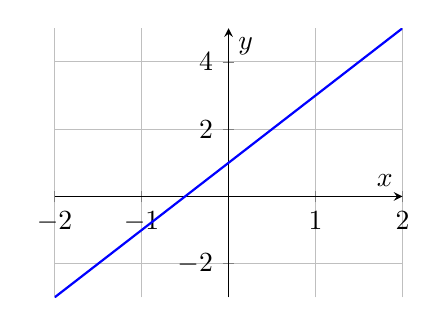
\begin{tikzpicture}
    \begin{axis}[
        axis lines = middle,
        xlabel = \(x\),
        ylabel = {\(y\)},
        samples = 100,
        domain=-2:2,
        grid=both,
        width=6cm,
        height=5cm,
    ]
    \addplot[blue, thick] {2*x + 1};
    \end{axis}
\end{tikzpicture}
  \caption{An example of a lineal function}
  \label{fig:example2}
\end{figure}


This is a linear function(Figure \ref{fig:example2}),  one of the simplest functions that can be viewed on calculus, sometimes a simple phenom can be viewed without getting in a huge amount of complexity and could be described with simple models, and when we have a problem or a situation in the reality when we need to create a machine hat can predict future data, what can we do?
In those cases, as it has been portrayed, a linear function can be used as a mathematical feature that attempts to fit on the data.
\begin{figure}[h]
\centering
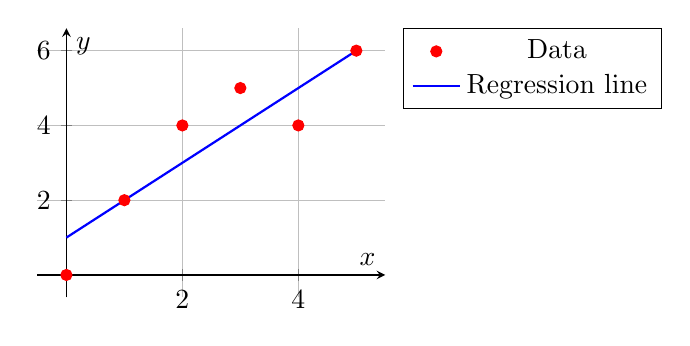
\begin{tikzpicture}
  \begin{axis}[
      axis lines = middle,
      xlabel = \(x\),
      ylabel = {\(y\)},
      grid = both,
      width = 6cm,
      height = 5cm,
      enlargelimits = true,
      legend style={at={(1.05,1)}, anchor=north west},
  ]
  \addplot[
      only marks,
      mark=*,
      color=red,
  ] table {
      0 0
      1 2
      2 4
      3 5
      4 4
      5 6
  };
  
  
  \addplot[
      domain=0:5, 
      samples=100, 
      color=blue, 
      thick
  ] {x + 1};
  
  \legend{Data, Regression line}
  
  \end{axis}
\end{tikzpicture}
  \caption{A simple example of a lineal regression}
  \label{fig:example3}
\end{figure}
Despite that nowadays exist several types of models that can predict future data, lineal regression as it is one of the simplest due to it just use a mathematical function that is easy to use, a lot of new models can be tested with a contraposition of lineal regression.
So, the Lineal regression is described as 
$$y=\beta_0x+\beta_1+e$$
$\beta_0$ it is the slope and $\beta_1$ is the intercept. And e is the error tha exist on the model.

However it'll be required to know some metrics that will help us to find out how efficient is our model and to know the error that we have in our model too\citep{bruce2020practical}
\begin{itemize}
  \item $R^2$: This metric can measure how much the model can describe the phenom. The $R^2 \in [0,1]$ and if the model tends to 1 the model can describe better the phenom and can be more precise in the predictions.
  \item $MSE$ and $RMSE = $ Are metrics that measure the distance between the value predict against the real value.
  $$MSE=\frac{1}{n}\Sigma^{n}_{i=1}(y_i-\hat{y}_i)^2 $$
    $$RMSE=\sqrt{\frac{1}{n}\Sigma^{n}_{i=1}(y_i-\hat{y}_i)^2} $$
    The difference between MSE and RMSE are that MSE is susceptible to detect outliers values due to the nature of a square function, and also it helps to know the variance that we got in our model. Nevertheless, RMSE use the same scale of the values and want to measure the error as it is on the data.

\end{itemize}

\subsection{Knn model}
It consist in to look out on the data and predict a value according to the vicinity of the values nearest from the data that is presented. Knn presents two basic hyperparameter, the first one is the number of vicinity and the second is the type of distance that it'll be chosen.
Knn model has some different parameters if we measure it as classifier. However at this case it'll be used the Knn model as a regressor, so it'll be usable the metrics that it has been described before.
(figure \ref{fig:example4})
\begin{figure}[H]
  \centering
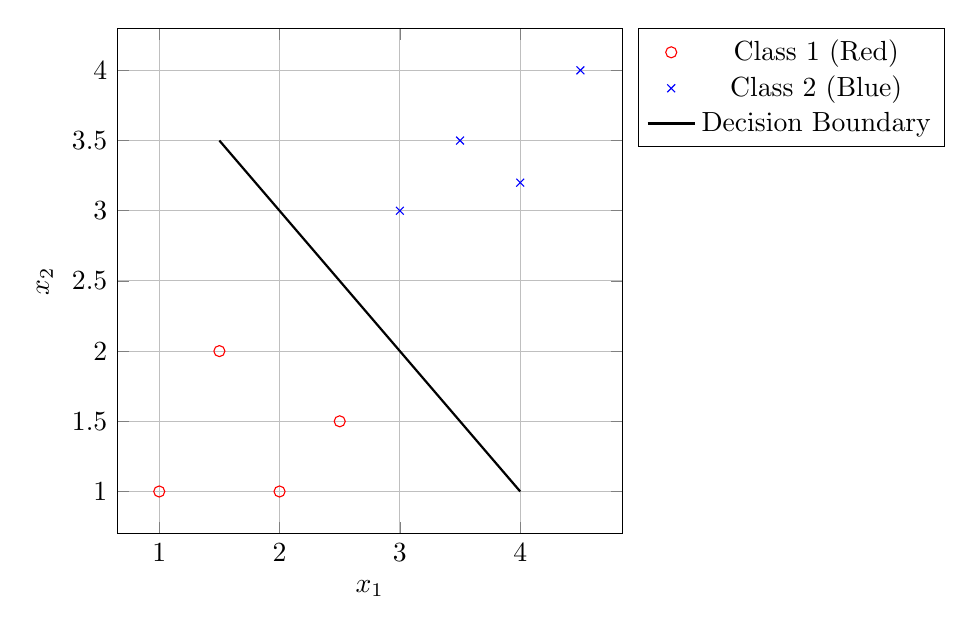
\begin{tikzpicture}
  \begin{axis}[
      width=8cm, height=8cm,
      xlabel={$x_1$},
      ylabel={$x_2$},
      grid=major,
      legend pos=outer north east,
      domain=0:5,
      samples=100
  ]
      % Define the coordinates of two classes
      \addplot[only marks, red, mark=o] plot coordinates {(1,1) (1.5,2) (2,1) (2.5,1.5)};
      \addplot[only marks, blue, mark=x] plot coordinates {(3,3) (3.5,3.5) (4,3.2) (4.5,4)};
      
      \addlegendentry{Class 1 (Red)}
      \addlegendentry{Class 2 (Blue)}
      
      % Plot decision boundary (simplified for K=1)
      \addplot [domain=1.5:4, samples=2, thick,range=3:1] {-x+5};
      \addlegendentry{Decision Boundary}
      
  \end{axis}
\end{tikzpicture}

  \caption{A simple example of knn regressor}
  \label{fig:example4}
\end{figure}
After knowing the main features that were used at this study, let's look out for the process that has been followed. As it'll have seen, the process aims to use the scientific method, however, with the features of a data analyst

\begin{tikzpicture}[node distance=2cm]
  
  % Nodes
  \node (start) [startstop] {Read the datasets};
  \node (process1) [process, below of=start] {Processing the data};
  \node (proccess2)[process, right of=process1, xshift=2cm]{Data exploration};
  \node (proccess3)[process, right of=proccess2, xshift=2cm]{Finding descriptive values and NaNs};
  \node (proccess4)[process, below of=proccess3]{Applying transformations};
  \node (proccess5)[process, left of=proccess4, xshift=-2cm]{Compare with metrics and plotting};
  \node (proccess6)[process, left of=proccess5, xshift=-2cm]{Create a regressor model and checking out the relevant metrics};
 
  \node (decision1) [decision, below of=proccess6, yshift=-2cm] {The model may be upgraded it?};
  \node (process2a) [process, below of=decision1, xshift=-4cm] {Check and reviewing with different perspectives};
  \node (decision2) [decision, below of=decision1, xshift=4cm] {My model is underfitted or overfitted?};
  \node (process3a)[process, below of=proccess6, xshift=4cm]{Compare it with Knn model};
  \node (process4a)[process, below of=decision2, xshift=4cm]{Make their confidence intervals and propose the model};
  \node (stop) [startstop, below of=process2a, yshift=-1cm, xshift=3cm] {Stop};
  
  % Arrows
  \draw [arrow] (start) -- (process1);
  \draw [arrow] (proccess6) -- (decision1);
  \draw [arrow] (process1) -- (proccess2);
  \draw [arrow] (proccess2) -- (proccess3);
  \draw [arrow] (proccess3) -- (proccess4);
  \draw [arrow] (proccess4) -- (proccess5);
  \draw [arrow] (proccess5) -- (proccess6);
  \draw [arrow] (proccess6) --  (process3a);
  \draw [arrow] (process3a) --  (decision1);
  
  \draw [arrow] (decision1) -- node[anchor=east,yshift=0.2cm] {Yes} (process2a);
  \draw [arrow] (decision1) -- node[anchor=west,yshift=0.2cm] {No} (decision2);
  \draw [arrow] (decision2) -- node[anchor=west,yshift=-0.2cm] {Yes} (process2a);
  \draw [arrow] (decision2) -- node[anchor=west,yshift=0.2cm] {No} (process4a);
  \draw [arrow] (process2a) |- (process1);
  \draw [arrow] (process4a) |- (stop);
  \end{tikzpicture}
  
  \begin{figure}[h]
  \caption{The procedural followed at the investigation}
  \label{fig:diagram}
  
\end{figure}

These were the main steps followed at the work. The part of reading some material and check information from several sources, is mainly the first step before to begin the work. However if there's something missing when the hypothesis are covered, it'll be useful to look for more sources to create other hypothesis.

\section{Data analysis}
\subsection{first dataset}
The first data analysis that has been studied was the dataset with synthetic data. As it had been mentioned, following the scientific methodology we look for the data and it started with a data exploration.
It obtained the following values 
\begin{table}[H]
\begin{center}
  \begin{tabular}{|c|c|c|}
    \hline
   parameter & y & x \\ \hline
   number of values & 506.000000 & 506.000000\\
   mean  &  22.528854  &  3.613524\\
   std   &   9.182176  &  8.601545\\
   minimum   &   5.000000  &  0.006320\\
   percentile $25$   &  17.025000  &  0.082045\\
   percentile $50$   &  21.200000  &  0.256510\\
   percentile $75$   &  25.000000 &   3.677083\\
   maximum   &  50.000000  & 88.976200\\
   \hline
  \end{tabular}
  \caption{Parameters}
\end{center}
\end{table}
Now that we have assured that the data are completed we can see the value of the mean and the 50 percentile are quite different, mostly on the variable x, it requires to be cleaned the data. Nevertheless, it is useful to check the correlation with variable x to y too.
The correlation matrix resulted on 
\begin{table}[H]
\begin{center}
  \begin{tabular}{|c|c|c|}
    \hline
      & y & x  \\ \hline
     y&  1.000000 & -0.389582 \\
     x & -0.389582  & 1.000000 \\
     \hline
  \end{tabular}
  \caption{Correlation}
\end{center}
\end{table}
\begin{figure}[h]
  \centering
  \includegraphics[width=0.65\textwidth]{data1_plot1.png}
  \caption{Exploratory data}
  \label{fig:ejemplo}
\end{figure}


The correlation is quite low between x,y. That means that it'll be hard to find a relation with the x and y with linear regression.
And also, something that we can notice with the plots that they are not normally distributed. The x-axis it seems more a exponential distribution than normal.
Other way to demonstrate it could making a hypothesis test and verifying it with a Shapiro-walk; it consist to propose a null hypothesis, that if the value of statistic is closer to 1 or great, it will reject the hypothesis, therefore the distribution doesn't follow a normal distribution. By other hand if we encounter a value smaller it will indicate is that probably the distribution follows a normal distribution. And also we have de p value that if is greater than 0.05 will indicate that is a normal distribution, in the opposite way it is a non-normal distribution.
The test concluded with a distribution of  $4.85*10^-28$ so it is not a normal distribution.
At this point we can choose several ways to follow
\begin{itemize}
  \item Trying to normalizing
  \item Trying with models more associated with exponential distributions or models that will no depend on the distribution.
  \item Infer with other features
\end{itemize} 
Due to the objectives of the work, the first attempt it'll be used.
At this dataset has been followed 4 approaches to look the efficiency of methods at the cleaning of the data.
However, it has been tested several types of transformations to check out if it'll be more useful the logarithm transformation according with the parameter of skew 
\begin{table}[H]
\begin{center}
  \begin{tabular}{|c|c|c|}
    \hline
     type-skew & x & y  \\ \hline
     original& 5.223148798243851&1.1109118502479587\\
     log&1.2692005882725572&-0.24563979611568673\\
     sqrt&2.024382103123676&0.4381663127860419\\
     1/x&-0.5772191040682719&1.9393215717506038\\
     box-cox&0.093649&\dots\\
     outliers&0.40335&1.058543\\
      \hline
  \end{tabular}
\end{center}
\caption{Skewness in different types of transformations}
\end{table}
It could seems some techniques are better however logarithm transformation has a better resolution in the skew of both variables.    
\subsection{First method}
The first approach to make a model was transforming with logarithm and making a cross validation
\begin{figure}[h]
  \centering
  \includegraphics[width=0.65\textwidth]{model_1.png}
  \caption{Lineal regression}
  \label{fig:example_1}
\end{figure}
And therefore it was contrasted with the Knn model, getting the next values
\begin{table}[H]
\begin{center}
  \begin{tabular}{|c|c|c|}
    \hline
     metric & Lineal regression & Knn \\ \hline
     $R^2$l& 35.488840060699256\%&43.57\\
     MSE&0.09611374428381783&0.11904\\
     RMSE&0.30971201639466434&0.33166\\
     \hline
    %
  \end{tabular}
  \caption{First table}
\end{center}
\end{table}
The model has been contrasted with both models and with the same cleaned data, as also trained at the same way respectively at the model 
However, the Lineal regressor has been predicting the data within the confidence.
For example, it added a value x on 2.3 and the result in y is 2.7534 
The confidence value on 95\% interval is  from $(2.172214750599946, 3.334689169873629)$
and it has been seen the value was fitted correctly.
The best parameters found on kNN was with 21 neighbors and manhattan distance
\begin{figure}[h]
  \center
  \includegraphics[width=0.65\textwidth]{data2_plot.png}
  \caption{Lineal regression with the intervals set}

  \label{fig:example_intervals}
\end{figure}
However it has been made a generalized model to linear regression in a set of dots (fig\ref{fig:example_intervals})
The equation for this model is 
$$y=-0.21773690693332431x+3.2542468461834333$$
\subsection{Second method}
The second approach it consisted to just transforming the value with logarithm without CV 5x2
\begin{table}[H]
\begin{center}
  \begin{tabular}{|c|c|c|}
    \hline
     metric & Lineal regression & Knn \\ \hline
     $R^2$& 15.0589474050694\%&43.57674995779635\%\\
     MSE&0.1127456496305317&0.11904364904719832\\
     RMSE&0.3357761897909554&0.33166\\
     \hline
  \end{tabular}
  \caption{Second model}
\end{center}
\end{table}
The values obtained are quite low, and the test of interval values with a random value it has been displayed 
\begin{center}

\begin{figure}[h]
  \center
  \includegraphics[width=0.65\textwidth]{model_2.png}
  \caption{Lineal regression with the confidence intervals}
  \label{fig:example_intervals}
\end{figure}
\end{center}
The random value tested was $x=2.3$ $ y=2.712267315$
The CI of  95\% for 2.3 $(2.1310301053631586, 3.2935045246368415)$
so the equation resulting is: $$y=3.28236728 -0.24786955x $$

Here it found with 21 neighbors but with cosine distance
\subsection{Third method}
The outliers were fixed with capping and flooring methods using the median
\begin{table}[H]
\begin{center}
  \begin{tabular}{|c|c|c|}
    \hline
     metric & Lineal regression & Knn \\ \hline
     $R^2$& 32.19327627743514\%&32.92025378085354\%\\
     MSE& 0.002590185931743603&0.09954163106601016\\
     RMSE&0.3097120163946644&0.3155021886\\
     \hline

  \end{tabular}
  \caption{Third method}

\end{center}
\end{table}
\begin{figure}[h]
  \center
  \includegraphics[width=0.65\textwidth]{model_3_3.png}
  \caption{Lineal regression with the confidence intervals}

  \label{fig:example_intervals_3}
\end{figure}
The random value tested was $x=0.4$ $ y=1.1624568760450196$
The CI of  95\% for 2.3 $(1.0655741648818118, 1.2593395872082274)$
so the equation resulting is: $$y=1.2573964360450196 -0.23734890073453882x $$

\subsection{fourth method}
The last methods were used at this model. And also the test of Knn, was a little bit different to due it has been included the type of distance
\begin{table}[H]
\begin{center}
  \begin{tabular}{|c|c|c|}
    \hline
     metric & Lineal regression & Knn \\ \hline
     $R^2$& 37.1 \%&38.88337562736399\%\\
     MSE& 0.08067515724063212&0.06685108607726611\\
     RMSE&0.2839075215367599&0.3155021886\\
     \hline
    
  \end{tabular}
\end{center}
\caption{The four method}
\end{table}
Although, for this search of parameters, it got the Minkowski dataset, and finally the value of the intervals and equation are described as 
The random value tested was $x=0.4$ $ y=3.1646101221355143$
The CI of  95\% for 2.3 $(2.624302151585808, 3.7049180926852205)$
so the equation resulting is: $$y=3.2466778431246275 -0.20516930247278303x $$

The methods were contrasted by the simplest model and also the intervals were obtained, however that section it comprehends the results discussion

And one of the most important things that it has obtained is this table that compiles all the metrics and parameters that has been obtaining
\begin{table}[h]
  \small 
  \setlength{\extrarowheight}{-2pt} 
  \begin{tabular}{|l|l|l|}
  \hline
  \textbf{Metric} & \textbf{model1} & \textbf{model2} \\
  \hline
  $R^2$ & 35.4\% & 15.05\% \\
  \hline
  MSE & 0.0961 & 0.1127 \\
  \hline
  RMSE & 0.3097 & 0.3358 \\
  \hline
  EQUATION & $y=-0.2177x+3.2542$ & $y=-0.2479x+3.2824$ \\
  \hline
  Adjusted $R^2$ & 36.7\% & 39.8\% \\
  \hline
  F-statistic & 147.1 & 267.1 \\
  \hline
  $P(F-statistic)$ & 5.97e-27 & 2.11e-46 \\
  \hline
  Log-Likelihood & -50.079 & -91.384 \\
  \hline
  AIC & 104.2 & 186.8 \\
  \hline
  BIC & 111.2 & 194.8 \\
  \hline
  std error & const=0.024, x=0.018 & const=0.019, x=0.015 \\
  \hline
  $\sigma$ & const=135.161, x=-12.128 & const=170.036, x=-16.343 \\
  \hline
  $P>\|t\|$ & const: 0.000, x: 0.000 & const: 0.000, x: 0.000 \\
  \hline
  Confidence Intervals & const=[3.2068, 3.3017]  & const=[3.2444, 3.3203] \\
  & x=[-0.2531, -0.1824] &x=[-0.2777, -0.2181]\\
  \hline
  Omnibus & 41.738 & 37.308 \\
  \hline
  Prob(Omnibus) & 0.000 & 0.000 \\
  \hline
  Jarque-Bera (JB) & 64.331 & 64.192 \\
  \hline
  Prob(JB) & 1.07e-14 & 1.15e-14 \\
  \hline
  Skew & 0.960 & 0.581 \\
  \hline
  Kurtosis & 4.553 & 4.570 \\
  \hline
  Durbin-Watson & 0.983 & 1.902 \\
  \hline
  Condition Number & 2.26 & 2.16 \\
  \hline
  \end{tabular}
  \caption{Model comparison 1 and 2}
  \label{tab:modelos12}
  \end{table}
  \begin{table}[H]
  
  \small
    \setlength{\extrarowheight}{-2pt} 

  \begin{tabular}{|l|l|l|}
  \hline
  \textbf{Metric} & \textbf{model3} & \textbf{model4} \\
  \hline
  $R^2$ & 32.193\% & 37.1\% \\
  \hline
  MSE & 0.014957 & 0.0807 \\
  \hline
  RMSE & 0.12224 & 0.2839 \\
  \hline
  EQUATION & $y=-0.30537x+1.85673$ & $y=-0.2052x+3.2467$ \\
  \hline
  Adjusted $R^2$ & 33.5\% & 36.8\% \\
  \hline
  F-statistic & 128.2 & 147.8 \\
  \hline
  $P(F-statistic)$ & 2.76e-24 & 4.72e-27 \\
  \hline
  Log-Likelihood & 181.27 & -32.091 \\
  \hline
  AIC & -385.5 & 68.18 \\
  \hline
  BIC & -351.5 & 75.25 \\
  \hline
  std error & const=1.8567, x=-0.3054 & const=0.022, x=0.017 \\
  \hline
  $\sigma$ & const=0.015, x=0.027 & const=144.464, x=-12.159 \\
  \hline
  $P>\|t\|$ & const: 0.000, x: 0.000 & const: 0.000, x: 0.000 \\
  \hline
  Confidence Intervals & const=[1.8279, 1.886] & const=[3.2024, 3.2909],  \\
  &  x=[-0.3584, -0.2522]&x=[-0.2384, -0.1719]\\
  \hline
  Omnibus & 40.637 & 35.555 \\
  \hline
  Prob(Omnibus) & 0.000 & 0.000 \\
  \hline
  Jarque-Bera (JB) & 56.377 & 46.953 \\
  \hline
  Prob(JB) & 5.73e-13 & 6.37e-11 \\
  \hline
  Skew & 1.021 & 0.938 \\
  \hline
  Kurtosis & 4.087 & 3.966 \\
  \hline
  Durbin-Watson & 0.966 & 0.958 \\
  \hline
  Condition Number & 4.45 & 2.26 \\
  \hline
  \end{tabular}
  \caption{Model comparison 3 and 4}
  \label{tab:modelos34}
  \end{table}


\subsection{Second dataset}
The next dataset that it has been studying was about cars. It is a car's magazine from 1985 that compiles prices and features from several cars. 
For this dataset it has been read some papers(include the cite) to understand some of the features and its relationship. 
As a one of the first steps was the cleaning the data, and a data exploration was made to look for missing values and 
\begin{center}
\begin{figure}[H]
  \center
  \includegraphics[width=1.1\textwidth]{heatmap.png}
  \caption{The heatmap of correlation}
  \label{fig:heatmap}
\end{figure}
\end{center}
The heatmap (Figure \ref{fig:heatmap}) represents how is related a variable with other. As the objective of the study is to making a model that can predict the price of cars according to certain variables. 
However a tool that can save time it is to see the correlation with continuous variables. So those variables that have been analyzed were the Curb weight, engine size, horsepower city-mpg and highway-mpg.
The procedure to clean up the data was the same as the previous dataset however some columns contained a few NaN values and they must be changed. As also, some features are measured by different magnitudes, for example, amounts of money and horse power, so it would useful to standardize the data and also it could be applied a logarithm transformation due to some the dataset wasn't following a normal distribution, instead it was a exponential distribution(figure \ref{fig:box},\ref{fig:box2}).
\begin{figure}[H]
  \centering
  \begin{minipage}[b]{0.5\textwidth}
      \centering
      \includegraphics[width=\textwidth]{box.png}
      \caption*{Example when the data is not standardized}
      \label{fig:box}
  \end{minipage}
  \begin{minipage}[b]{0.5\textwidth}
      \centering
      \includegraphics[width=\textwidth]{box2.png}
      \caption*{Example when data is standardized and transformed}
      \label{fig:box2}
  \end{minipage}
\end{figure}
\subsection{Engine size}
\begin{table}[H]
\begin{tabular}{|c|c|c|}
  \hline
   metric & Lineal regression & Knn \\ \hline
   $R^2$& 73.62087367142167 \%&78.14960577066459\%\\
   MSE& 0.00992703573774292&0.008260694761950247\\
   RMSE&0.09960553714701531&0.09078358735816178\\
   \hline
  \end{tabular}
  \caption{Engine size}
\end{table}
Prediction for x=0.9: 0.873558685297521

Ci of  95\%for x=0.9: (0.6755512178129525, 1.0715661527820897)
$$y=1.0421234211972827x-0.06435239378003343$$
The best parameters obtained were with Minkowski distance with 10 neighbors,  value of $p=1$ and the weight was according with the distance 
\subsection{Miles per gallon on city }
\begin{table}[H]
\begin{tabular}{|c|c|c|}
  \hline
   metric & Lineal regression & Knn \\ \hline
   $R^2$& 60.45640689950125 \%&63.98078808830601\%\\
   MSE&0.020279279592056144&0.01864935309235264\\
   RMSE&0.14237431771458053&0.13622653661454523\\
   \hline
  \end{tabular}
  \caption{ Miles per gallon on city}
\end{table}
Prediction for x=0.9: 0.001530863668857796

Ci of 95\%for x=0.9: (-0.2679841644933157, 0.2710458918310313)
$$y=-0.847735376275263x+0.7644927023165945$$
%%
The best parameters obtained were with Minkowski distance with 10 neighbors,  value of $p=1$ and the weight was uniform
\subsection{Highway miles per gallon }
\begin{table}[H]
\begin{tabular}{|c|c|c|}
  \hline
   metric & Lineal regression & Knn \\ \hline
   $R^2$& 60.26238063837296 \%&71.4051650378093\%\\
   MSE&0.020296748345956392&0.01473467535564263\\
   RMSE&0.14246665691899474&0.12126069885616314\\
   \hline
  \end{tabular}
  \caption{ Highway miles per gallon}
\end{table}
Prediction for x=0.9: 0.029920806311725112

Ci of  95\%for x=0.9: (-0.23756924465403179, 0.297410857277482)
$$y=-0.8749508264218194x+0.8173765500913626$$
The best parameters obtained were with Minkowski distance with 5 neighbors,  value of $p=1$ and the weight was uniform
%%
\subsection{Curb weight}
\begin{table}[H]
\begin{tabular}{|c|c|c|}
  \hline
   metric & Lineal regression & Knn \\ \hline
   $R^2$& 75.95183149109518 \%&75.37829642479748\%\\
   MSE&  0.012140499045124736& 0.012413594738192302\\
   RMSE&0.10997951973411302
   &0.11115941370057997\\
   \hline
  \end{tabular}
  \caption{ Curb weight}
\end{table}
Prediction for x=0.9: 0.8331700416235279
Ci of  95\%for x=0.9: (0.6006405680156519, 1.065699515231404)
$$y=0.9548221722260348x -0.026169913379903483$$

The best parameters obtained were with Minkowski distance with 5 neighbors,  value of $p=1$ and the weight was uniform
\begin{table}[H]
\subsection{Horse power}
\begin{tabular}{|c|c|c|}
  \hline
   metric & Lineal regression & Knn \\ \hline
   $R^2$& R²: 69.07940114232951 \%&76.03392244337541\%\\
   MSE&  0.018231972174382657& 0.012141600878739993\\
   RMSE&0.1350239468208517& 0.11008958256719932\\
   \hline
  \end{tabular}
  \caption{ Horse power}
\end{table}
Prediction for x=0.9: 0.8188622328838921

Ci of  95\%for x=0.9: (0.5575508676925711, 1.0801735980752132)
$$y=0.8850130631724356x +0.022350476028700144$$

The best parameters obtained were with Minkowski distance with 5 neighbors,  value of $p=1$ and the weight was according to the distance
\subsection{Make}
\begin{table}[H]
\begin{tabular}{|c|c|c|}
  \hline
   metric & Lineal regression & Knn \\ \hline
   $R^2$& 64.3410145660548 \%&57.88546475881029\%\\
   MSE&  0.010664898715086689&  0.021450305579098994\\
   RMSE&0.018231972174382653&0.14644366261328212
   \\
   \hline
  \end{tabular}
  \caption{ Make}
\end{table}
Prediction for x=0.7: 9.776875346817139

Ci of 95\%for x=0.9: (9.502410532700683, 10.051340160933595)
$$y=0.18958328x +9.644167050817138$$
The best parameters for Knn obtained were with Hamming distance with 5 neighbors and the weight was according to the distance

This model it has to be taken with careful due to is a colinear model that has a several brands of cars. At also, the slopes are


slopes=0.18958328,0.50766223 ,-1.26198477, -0.99000114 ,-0.92894517, -0.6305545,
1.16321074, -0.68259389,  1.23056047 , 0.09693613, -0.91120827, -0.65395334
-0.00913223, -0.95232464 , 0.75358479, -0.68607991,  0.0266443,  -0.99147226,
-0.65961111, -0.6527091 ,  0.27815024


The way that it has been chosen the categorical variable of Make than the other variables, it is because they were tested with ANOVA, and the statistical significance
\begin{table}[h]
  \centering
  \scriptsize
  \setlength{\extrarowheight}{2pt} 
  \begin{tabular}{|l|c|c|c|c|}
  \hline
  \textbf{Categoric} & \textbf{Square sum (sum\_sq)} & \textbf{degree freedom (df)} & \textbf{F} & \textbf{Value PR(>F)} \\ 
  \hline
  \textbf{make}       & 9.750960e+09 & 21.0 & 29.502216 & 1.019818e-47 \\
  \textbf{fuelType}   & 1.534125e+08 & 1.0  & 2.495859  & 0.115703 \\
  \textbf{aspiration} & 3.969954e+08 & 1.0  & 6.587290  & 0.010991 \\
  \textbf{numofdoors} & 2.672851e+07 & 1.0  & 0.427171  & 0.514127 \\
  \textbf{body}       & 1.960055e+09 & 4.0  & 9.183927  & 7.844576e-07 \\
  \textbf{drive}      & 5.060130e+09 & 2.0  & 67.503667 & 3.539271e-23 \\
  \textbf{engineloc}  & 1.383992e+09 & 1.0  & 24.979629 & 0.000001 \\
  \textbf{type}       & 2.538008e+09 & 6.0  & 8.298116  & 5.008078e-08 \\
  \textbf{cylinders}  & 7.336567e+09 & 6.0  & 45.727054 & 7.149270e-35 \\
  \textbf{system}     & 4.352758e+09 & 7.0  & 14.797402 & 1.865735e-15 \\
  \hline
  \end{tabular}
  \caption{ ANOVA Results with the value PR($>$F) for categorical differences.}
  \label{tab:anova_results}
  \end{table}
  \begin{figure}[H]
    \centering
    \begin{minipage}[b]{0.3\textwidth}
        \centering
        \includegraphics[width=\textwidth]{image1.png}
        \caption*{Engine size regressor}
    \end{minipage}
    \begin{minipage}[b]{0.3\textwidth}
        \centering
        \includegraphics[width=\textwidth]{image2.png}
        \caption*{Miles per gallon city}
    \end{minipage}
    \begin{minipage}[b]{0.3\textwidth}
        \centering
        \includegraphics[width=\textwidth]{image3.png}
        \caption*{Highway miles per gallon}
    \end{minipage}

    \vspace{0.5cm} 

    \begin{minipage}[b]{0.3\textwidth}
        \centering
        \includegraphics[width=\textwidth]{image4.png}
        \caption*{Curb weight}
    \end{minipage}
    \begin{minipage}[b]{0.3\textwidth}
        \centering
        \includegraphics[width=\textwidth]{image5.png}
        \caption*{Horse power}
    \end{minipage}
    \begin{minipage}[b]{0.3\textwidth}
        \centering
        \includegraphics[width=\textwidth]{image6.png}
        \caption*{Make}
    \end{minipage}
\end{figure}
Another thing to take in mind is the tendency that follows tha variables
\begin{figure}[H]
  \centering
  \begin{minipage}[b]{0.3\textwidth}
      \centering
      \includegraphics[width=\textwidth]{t1.png}
      \caption*{Curb weight and brand}
      \label{fig:t}
  \end{minipage}
  \begin{minipage}[b]{0.3\textwidth}
      \centering
      \includegraphics[width=\textwidth]{t2.png}
      \caption*{Engine size and brand}
      \label{fig:t2}
  \end{minipage}
  \begin{minipage}[b]{0.3\textwidth}
    \centering
    \includegraphics[width=\textwidth]{t3.png}
    \caption*{Prices and brand}
    \label{fig:t3}
\end{minipage}
\end{figure}
\section{Discussion}
\subsection{First data-set}
As we can observe on the table \ref{tab:modelos12} and table \ref{tab:modelos34} it proposed 4 different models with different type of data cleaning, however we have seen different results in each one. If we see the $R^2$ of the models the worst is the second model, and also, as it saw in the tables from each table, the value of the Knn and The regressor is the lowest although, is close among them. The best $R^2$ and also, it has a one of the closest values with Knn regressor, is the fourth model.
Now in terms of MSE and RMSE the third model had a lowest MSE and RMSE but the fourth model it has also a good resolution in that terms.
Always in Data science it can be created different models to represent different phenoms or different aims. In this case, we have seen that despite that the fourth model doesn't have the best MSE and RMSE from all models however it is no the worst, the percentage of describing data is the highest so if we have this model with just this two variables and type of regressor, it can choose the fourth model. However the best thing that it can be done on this dataset could it be use different models or different treatments on the distribution
\subsection{Second data-set}
In base on the related works, \citep{article_1012052} used a similar approach in the creation of the model and also at the prediction of price of cars. And here it found that the cars with a certain make have more influence in a price than cars with a unknown brand. And \citep{WOS:000927105100001} the way to describe different features that can lead to different prices of car int the Van regions had a similarity workflow than this work. As also they used similar metrics. And \citep{WEBER2019109} they found how the fuel consumption has a huge weight into the prices of cars. As also the make is other important factor to see.
In the last analysis, it could have seen that the main features had a strong relation were those related with the motor and the structure of the car. And also the efficiency of the combustion of fuel. In the case of categorical variables, the variable that had a better resolution in predictions was the make, so here it can be refuted the past works. To indicate the best model in terms of the car's infrastructure; could be the curb weight because it had a $R^2$ of 75\% and its Knn model has  similar approach,. Also its MSE and RMSE despite that is not the best of all, it is second model that has a good resolution on MSE and RMSE with values of 0.0121 and 0.109 respectively.
however, if it can be checked with the last tables,the engine size appear to be the most relevant when it is applied a knn model with 78.149\% as $R^2$ and with the lowest MSE and RMSE of 0.00820 and 0.0907.
So, as a linear regressor model the variable Curb weight is the best one, however, as the variable with the highest efficiency it is engine size, so this variable is the most significant 

These variables which are related with the structure of the car, tend to follow the mark and the prices respect to the mark has a similar approach. So it can be deduce that relevant and expensive cars would try to make their cars as better as possible, such in the efficiency of consumption of fuel or the curb weight, horse power. Meanwhile those brands that has a cheaper cost don't tend to have the better structure features.(figure\ref{fig:t},\ref{fig:t2},\ref{fig:t3})  
\section{Conclusions and future work}
In both datasets can be used other type of models and see its efficiency in the prediction, as also it could be useful try to use regressions that are more associated with exponential distributions. In the second part it could aim to see the colineality and compare the $R^2$ obtained in the last models respect to the colinear model. And also, the way that was cleaned the dataset could it be changed or taking other parameters in the Knn model. 
To make a good analysis it can be challenging because several variables could be related among them, but when it makes an analysis the best way to know if it is following the correct path is looking for related works and its results, with this as priority it could be good help to delimitate the variables to use as the models or the cleaning process.
\bibliographystyle{apalike}
\bibliography{references}

\end{document}
